% Beamer template
% Author: Ozgur Taylan TURAN
% Delft University of Technology

\documentclass[aspectratio=169]{beamer}
\usepackage{/home/taylanot/texmf/tex/beamerthemetot}
% PACKAGES
\usepackage[english]{babel}
\usepackage{graphicx}
\usepackage{animate}
%\usepackage{calc}
\usepackage{calligra}
\usepackage[absolute,overlay]{textpos}
\usepackage[T1]{fontenc}
%\usefonttheme{serif}
\usefonttheme{professionalfonts}
\usepackage{amsmath}
\usepackage{palatino}
\usepackage{mathpazo}
\usepackage{graphicx}
%\usepackage{subfig}
\usepackage{tikz}
\usetikzlibrary{shapes,arrows}
\usepackage{xcolor}
\usepackage[T1]{fontenc}
%\usefonttheme{serif}
%\usepackage{titling}
\usepackage{graphicx}
%\usepackage{subfig}
%\usepackage{tikz}
%\usetikzlibrary{shapes,arrows}
\usepackage{mathtools}
\usepackage{cancel}
    
% BIB SETTINGS
\usepackage[backend=bibtex,firstinits=true,maxnames=30,maxcitenames=20,url=false,style=authoryear]{biblatex}
\bibliography{../../../archive_bib/library.bib}

\setlength\bibitemsep{0.3cm} % space between entries in the reference list
\renewcommand{\bibfont}{\normalfont\scriptsize}
\renewcommand{\cite}[1]{\footnote<.->[frame]{\fullcite{#1}}}
\setbeamertemplate{bibliography item}{}

\setbeamertemplate{navigation symbols}{} % remove navigation symbols

\usepackage{perpage} \MakePerPage{footnote}

 % COVER PAGE INFO   
\newcommand{\mytitle}{\color{White}\huge{\textbf{Bessa Talks-Unofficial Meeting}}}
\newcommand{\mysubtitle}{\color{Pink}\Large{\textbf{A Brief History of F3DASM}}}
\newcommand{\myauthor}{\color{White}\textcalligra{\LARGE Ozgur Taylan Turan}}
\newcommand{\authorlabel}{\small O.T. Turan}
\author{\authorlabel}


\begin{document}
% COVER PAGE
{
{
\def\beamer@entrycode{\vspace*{-\headheight}}
\setbeamertemplate{frametitle}[default][center]
\setbeamertemplate{navigation symbols}{}
\usebackgroundtemplate{
\includegraphics[width=\paperwidth,height=\paperheight]{cover/coverart.pdf}}

\begin{frame}[plain] 

\begin{minipage}{\textwidth}
	\centering{\mytitle} \\
	%\vspace{1cm}
	%\centering{\mysubtitle} \\
	\vspace{1cm}
	\centering{\color{White}November 15, 2021} \\
	\vspace{1cm}
	\centering{\myauthor}\\
\end{minipage}
\end{frame}
}

\setbeamercovered{transparent}
\setbeamertemplate{footline}{\usebeamertemplate*{minimal footline}}
\setbeamertemplate{headline}{\usebeamertemplate*{minimal headline}}
\def\beamer@entrycode{\vspace*{-\headheight}}
}
% MAIN
\setbeamercovered{transparent}

\begin{frame}
  \centering
  \mysubtitle
\end{frame}

\begin{frame}
  \centering
  \color{Pink} Who is familiar with F3DASM?
\end{frame}

\begin{frame}
  \centering
  \color{Pink} Who is using or intends to use F3DASM?
\end{frame}


\begin{frame}{Data-Driven Design/Modeling}
  \centering
  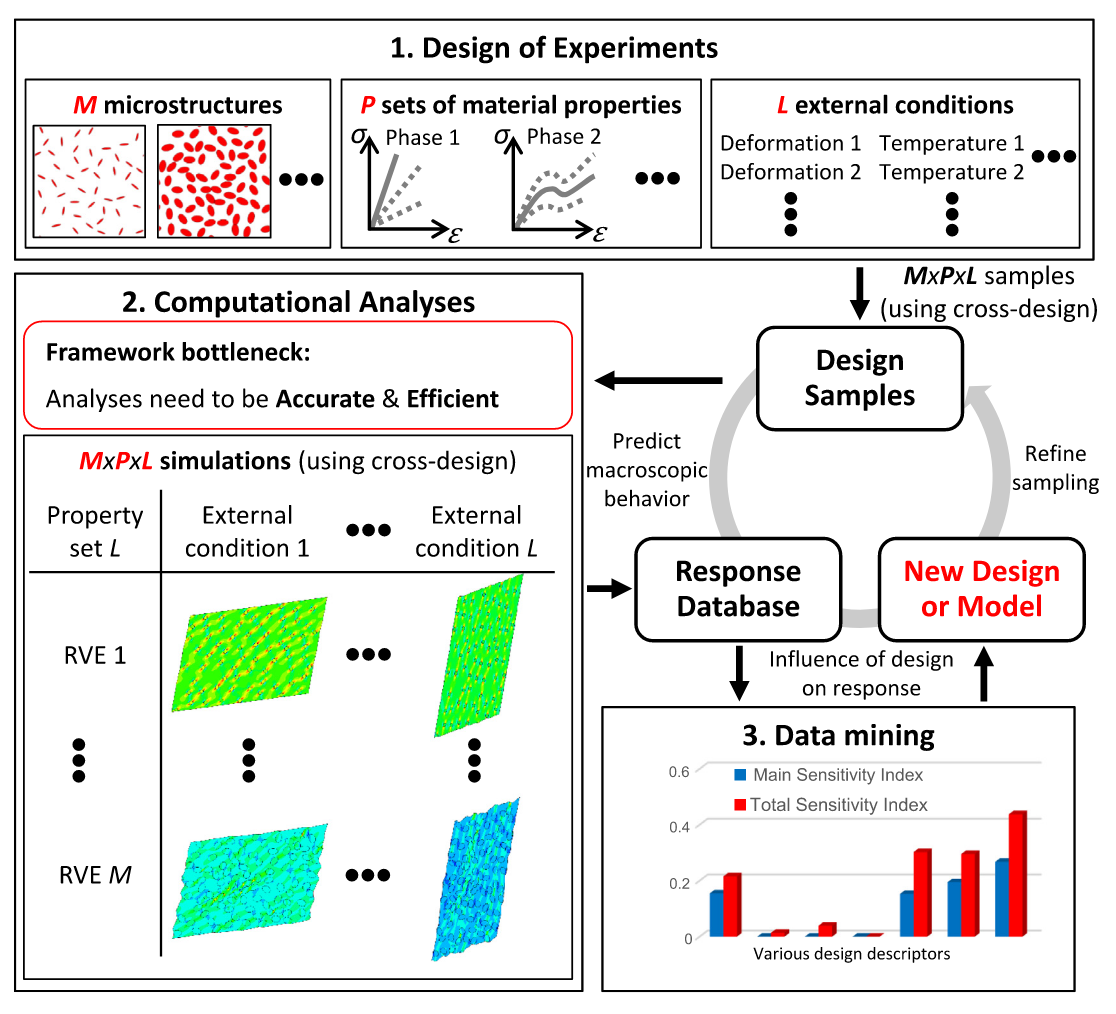
\includegraphics[height=0.8\textheight]{Figures/DDD.png}
\end{frame}

\begin{frame}{F3DAS}
  \begin{minipage}{0.5\textwidth}
  \begin{itemize}
    \item MATLAB$\to$ ABAQUS/Python-API for Simulation
    \item ML: Python 
  \end{itemize}
  \end{minipage}%
  \begin{minipage}{0.5\textwidth}
    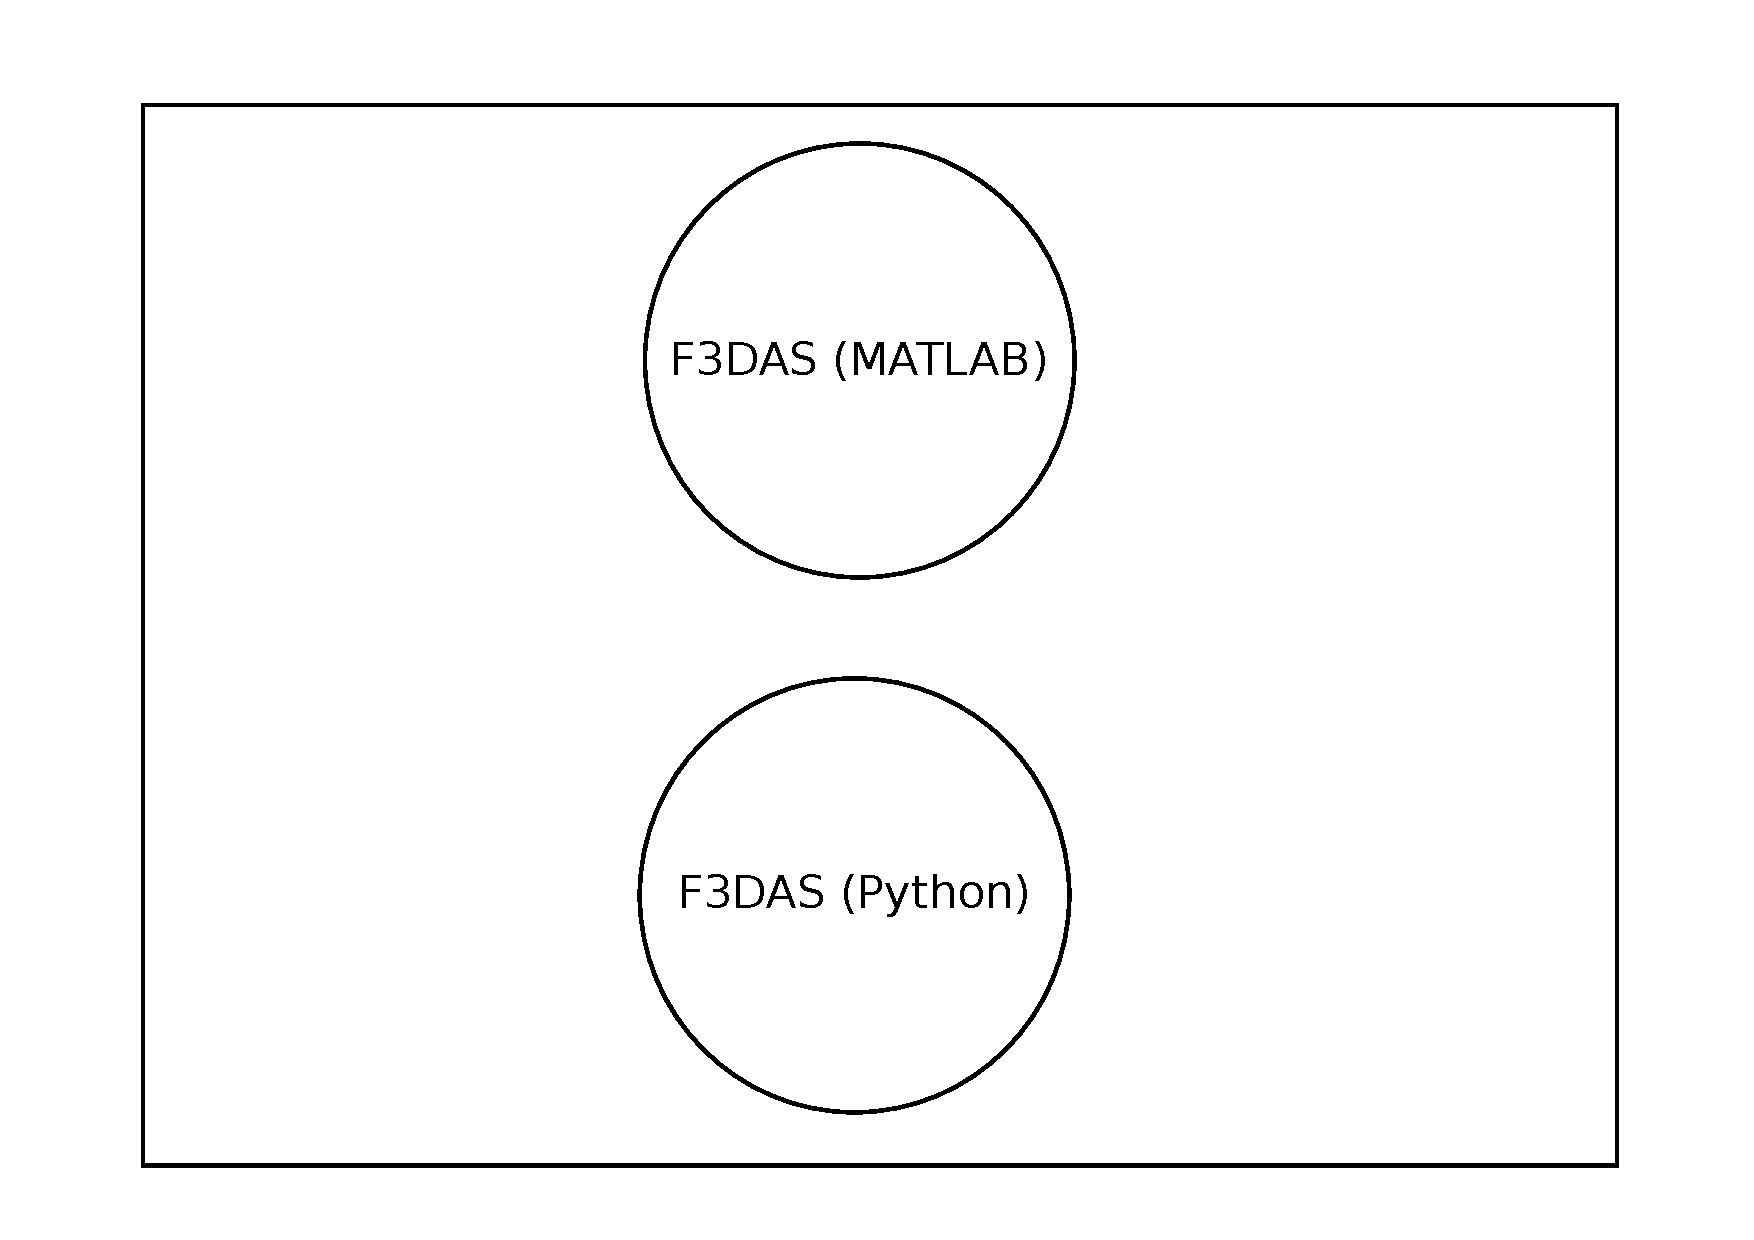
\includegraphics[width=\textwidth]{Figures/F3DAS.pdf}
  \end{minipage}
\end{frame}

\begin{frame}{F3DASM-v0.0.1}
  \begin{minipage}{0.5\textwidth}
  \begin{itemize}
    \item Luis$\to$ OOP Abaqus-PythonAPI ToolBox + SALib Interface
    \item Embedded implementations of Miguel's papers.
    \item ML: Separate python toolbox
  \end{itemize}
  \end{minipage}%
  \begin{minipage}{0.5\textwidth}
    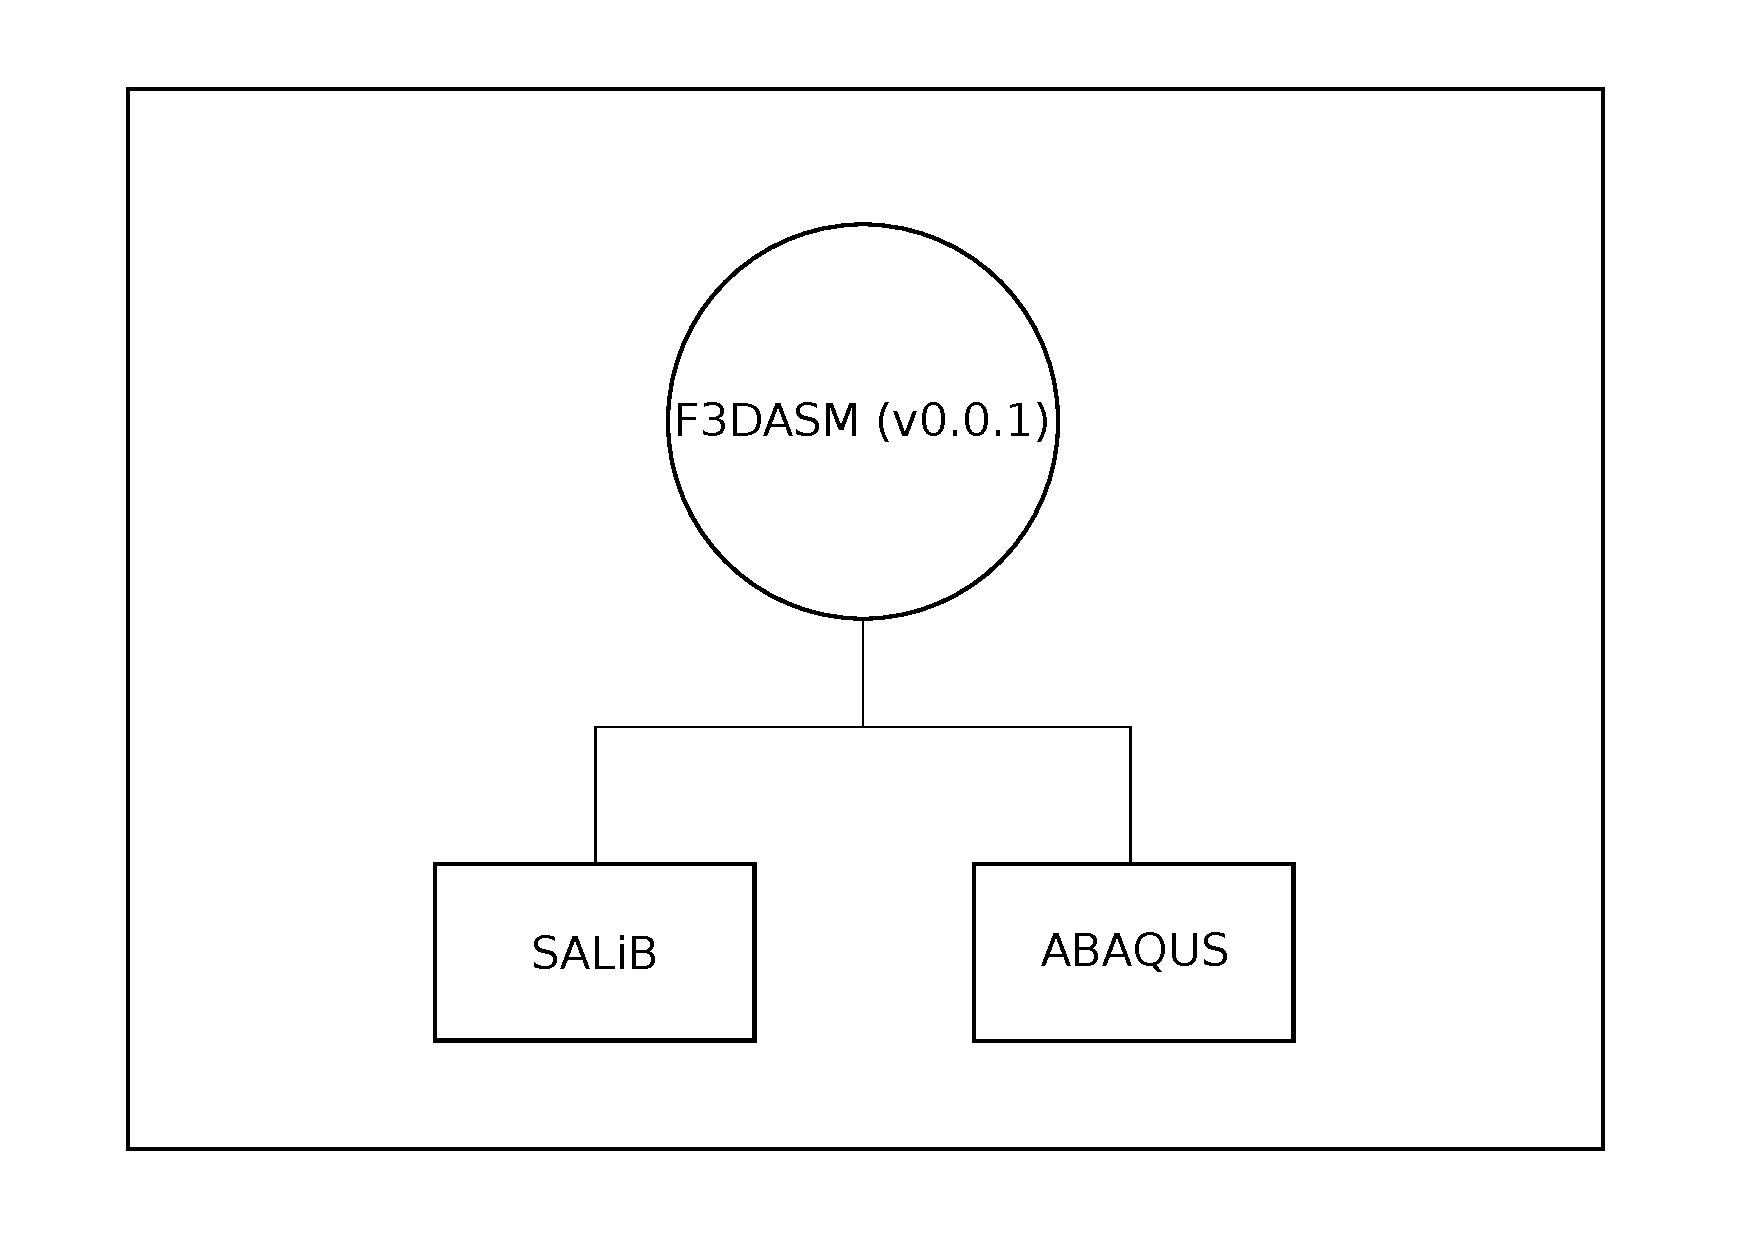
\includegraphics[width=\textwidth]{Figures/F3DASMv001.pdf}
  \end{minipage}
\end{frame}

\begin{frame}{F3DASM2}
  \begin{minipage}{0.5\textwidth}
  \begin{itemize}
    \item<1> Lightweight abstracted work-tree
    \item<2> No embedded implementation by itself, just thin wrappers to your hardcore projects/toolboxes
  \end{itemize}
  \end{minipage}%
  \begin{minipage}{0.5\textwidth}
    \includegraphics<1>[width=\textwidth]{Figures/F3DASM2.pdf}
    \includegraphics<2>[width=\textwidth]{Figures/F3DASM2-extra.pdf}
  \end{minipage}
\end{frame}

\begin{frame}{F3DASM2}
  \begin{minipage}{0.5\textwidth}
    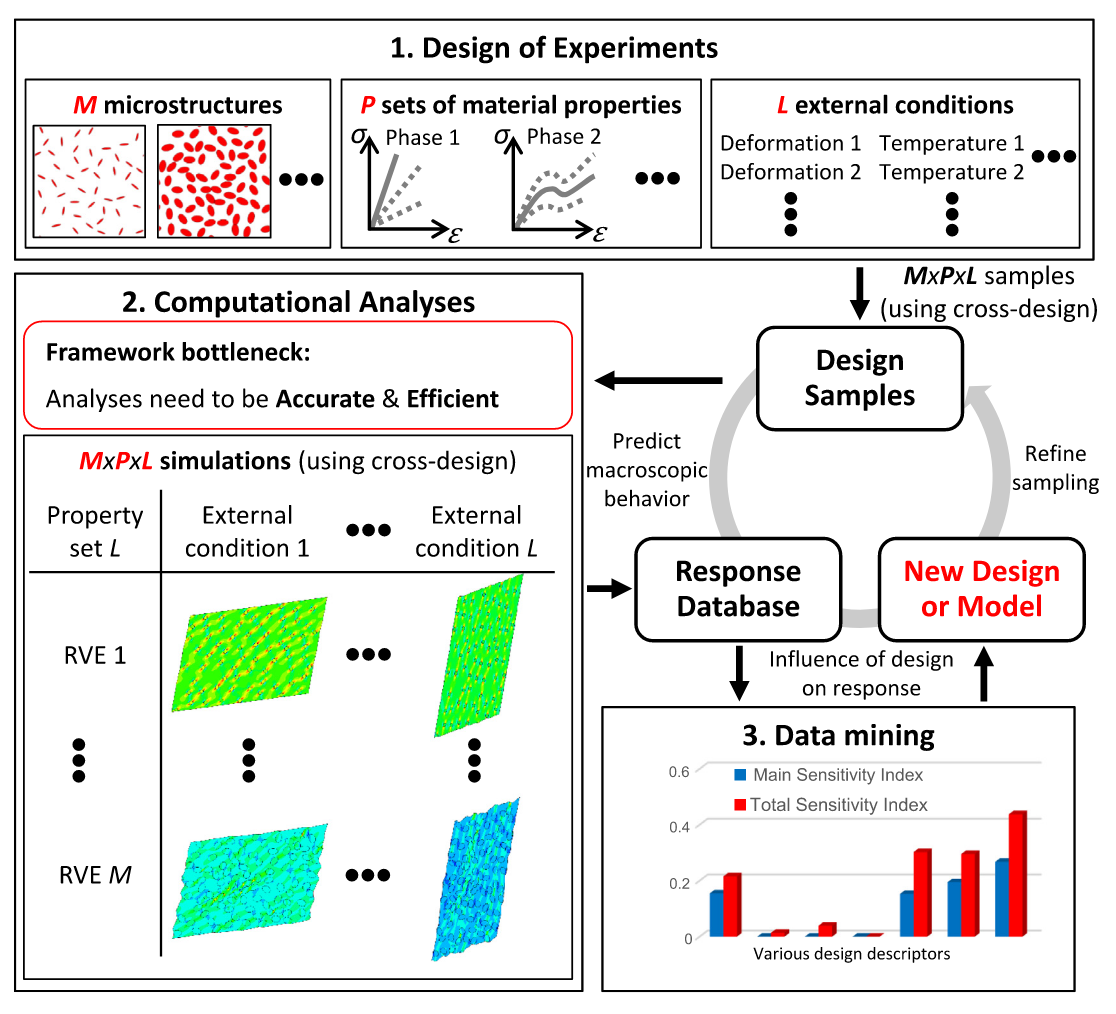
\includegraphics[width=\textwidth]{Figures/DDD.png}
  \end{minipage}%
  \begin{minipage}{0.5\textwidth}
    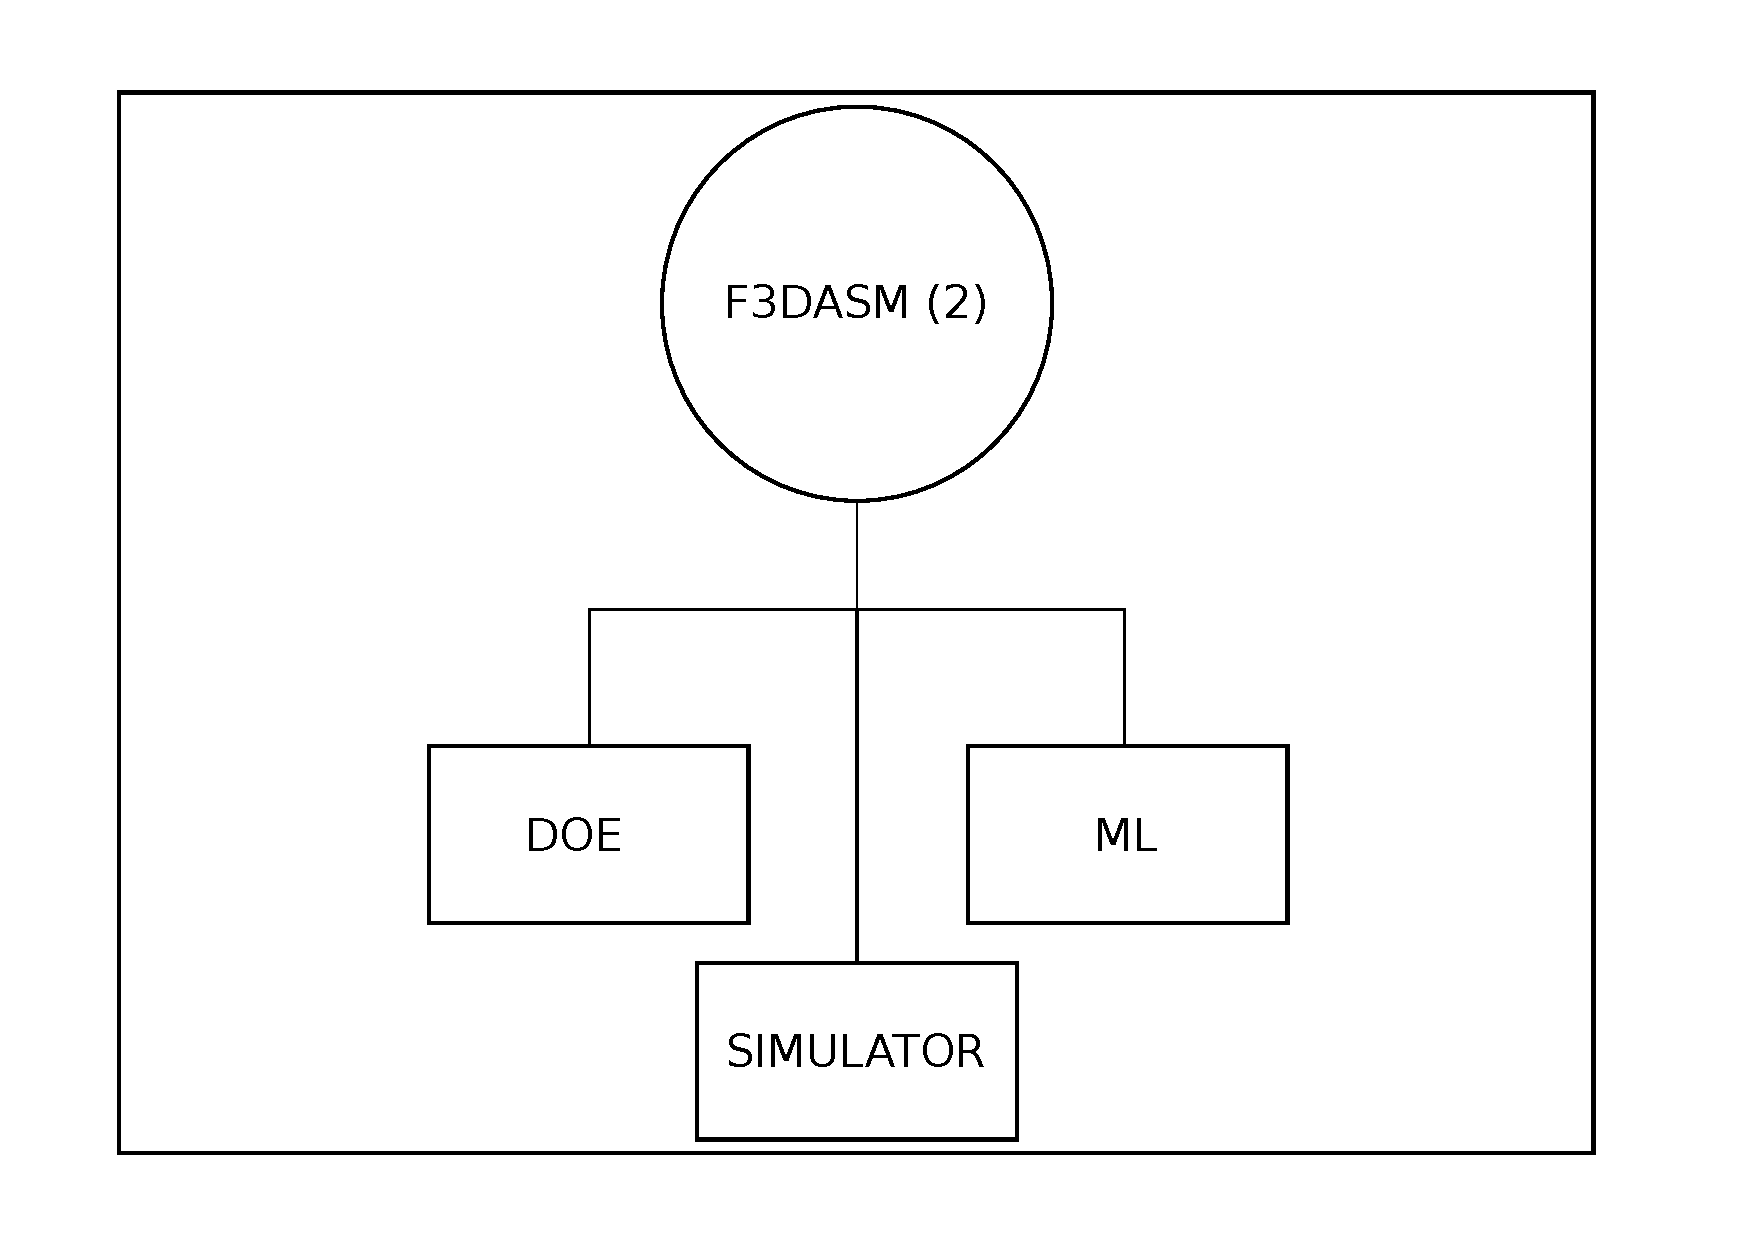
\includegraphics[width=\textwidth]{Figures/F3DASM2.pdf}
  \end{minipage}
\end{frame}

\begin{frame}{F3DASM-LatestDevelopmentBranch}
  \begin{minipage}{0.5\textwidth}
  \begin{itemize}
    \item Shushu (FENiCS) and Gawel (ABAQUS)
    \item Follows the basic ideology of F3DASM2
    \item Embedded models in F3DASM repo (gmshModel?)
    \item Separate Machine Learning 
  \end{itemize}
  \end{minipage}%
  \begin{minipage}{0.5\textwidth}
    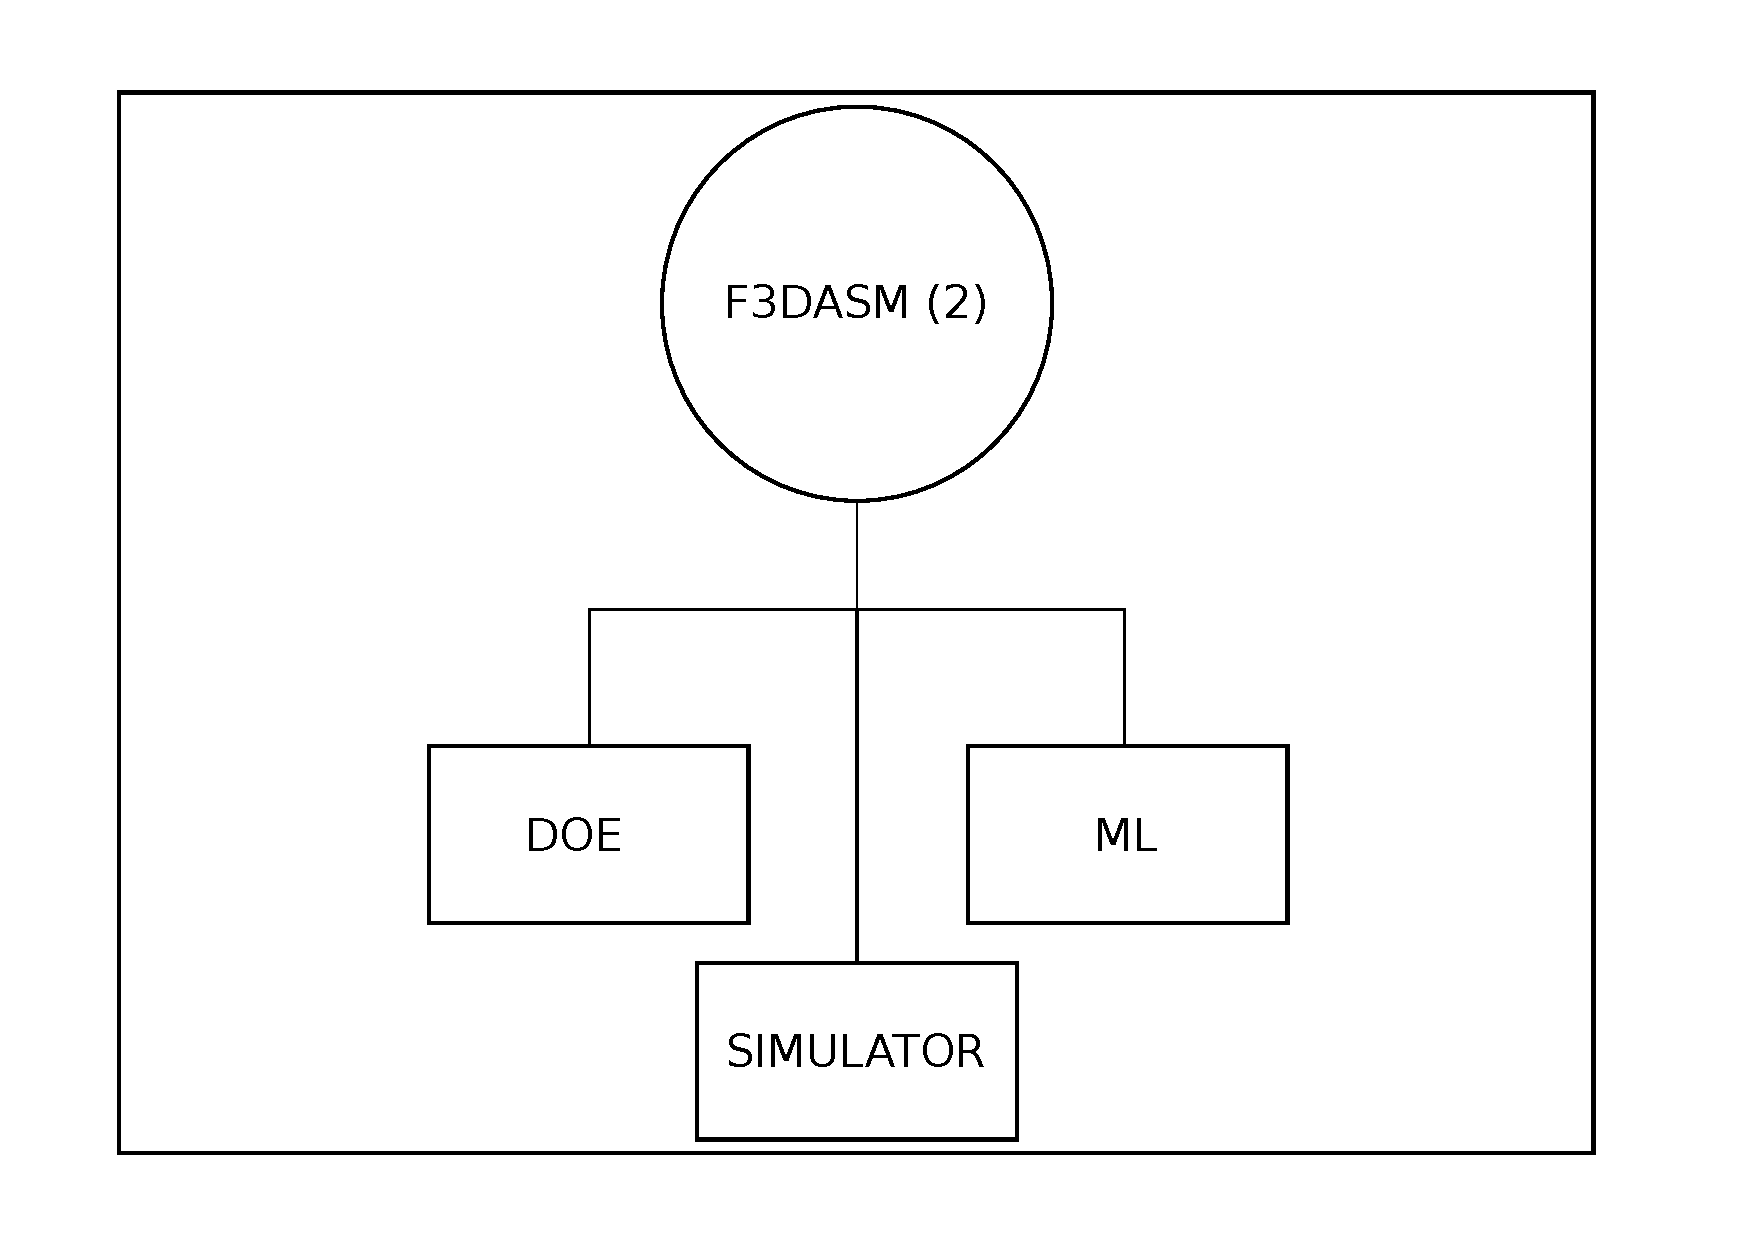
\includegraphics[width=\textwidth]{Figures/F3DASM2.pdf}
  \end{minipage}
\end{frame}

\begin{frame}{DDSCT-v0.0.1}
  \begin{minipage}{0.5\textwidth}
  \begin{itemize}
    \item Another skeleton implementation of F3DASM
    \item Miguel's commentary
    \item Utilization by MSc. students in the future
    \item Ready for deploy models
  \end{itemize}
  \end{minipage}%
  \begin{minipage}{0.5\textwidth}
    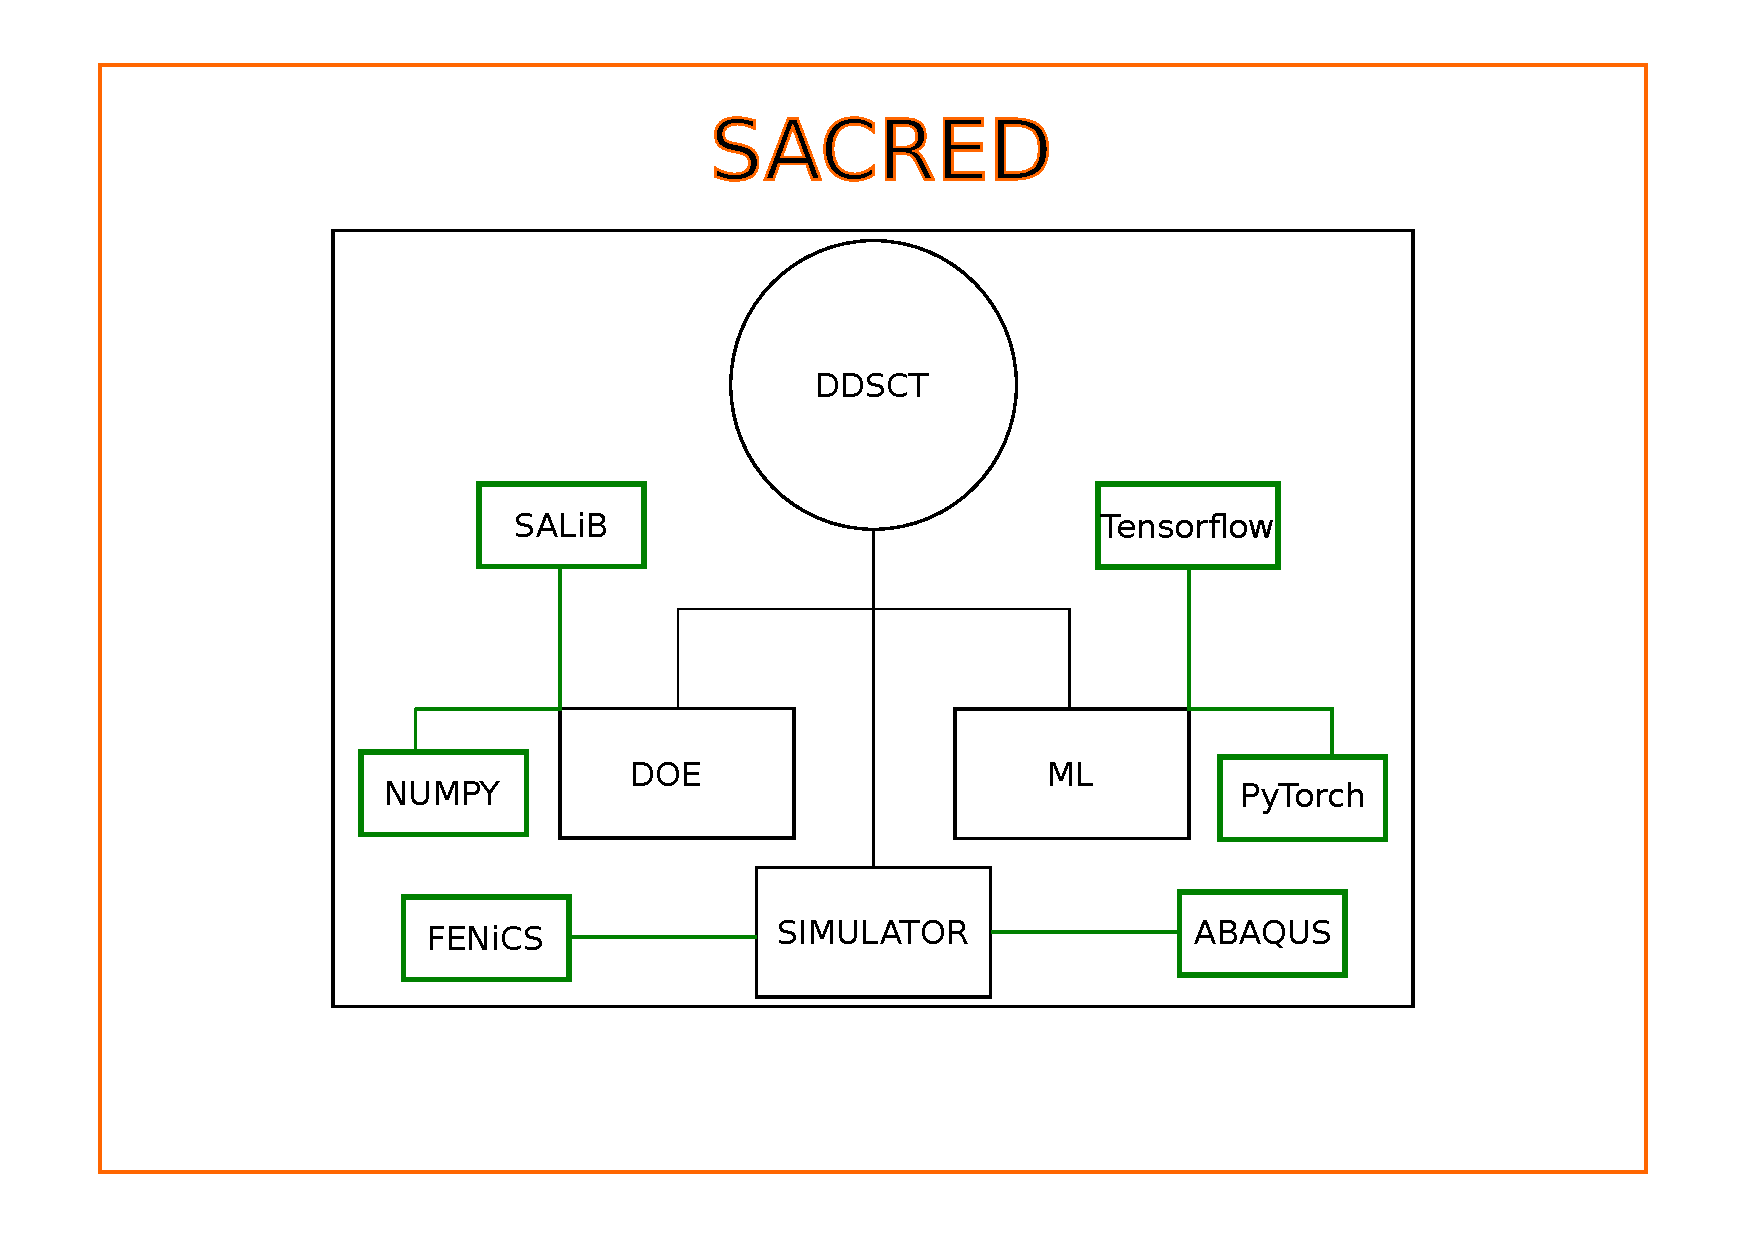
\includegraphics[width=\textwidth]{Figures/DDSCT.pdf}
  \end{minipage}
\end{frame}

\begin{frame}{DDSCT-v0.0.1}
  \begin{minipage}{0.5\textwidth}
    \begin{block}{\color{White} Sacred}
  \begin{itemize}
    \item Directory handling
    \item Configure/log/reproduce
    \item JIT compiler benefits
  \end{itemize}
    \end{block}
  \end{minipage}%
  \begin{minipage}{0.5\textwidth}
    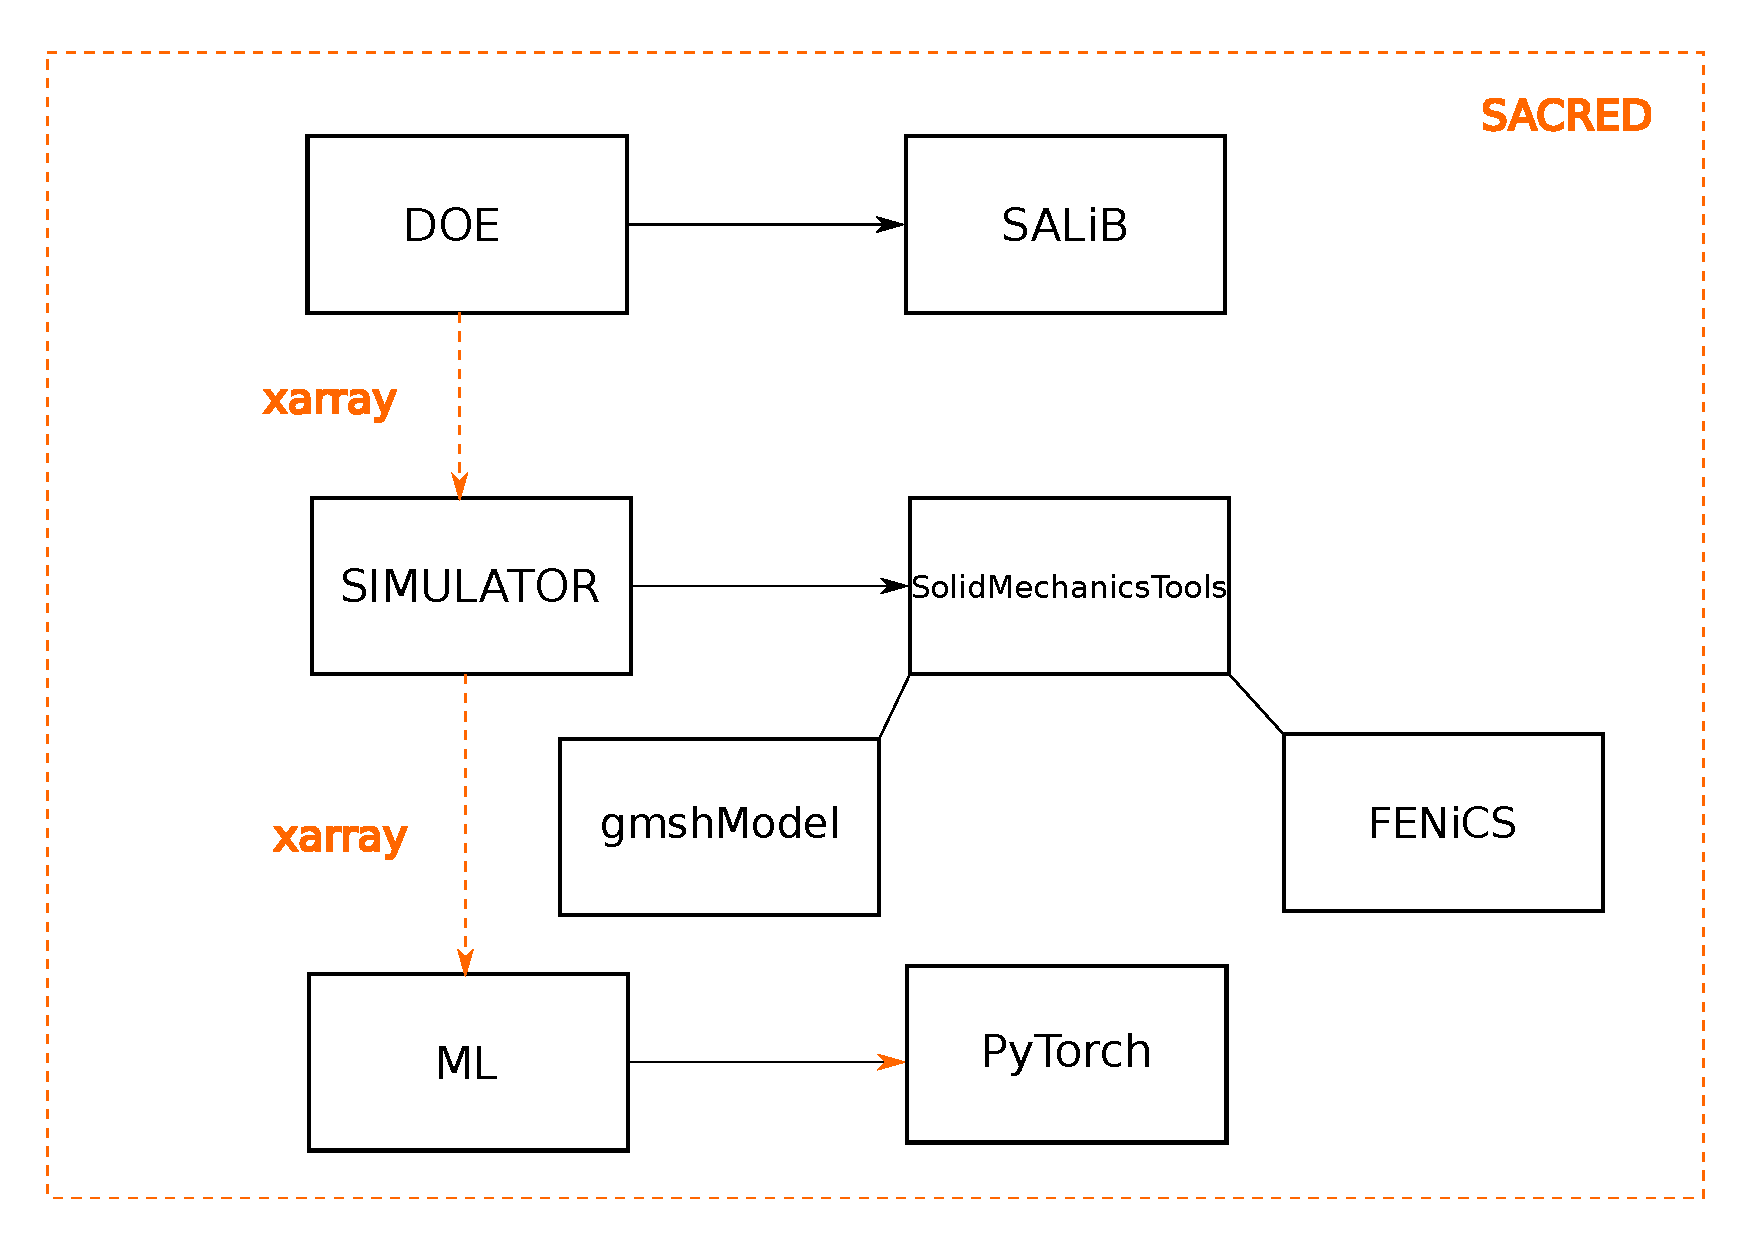
\includegraphics[width=\textwidth]{Figures/DDSCT-flow.pdf}
  \end{minipage}
\end{frame}

\begin{frame}{DDSCT-v0.0.1}
  \begin{minipage}{0.5\textwidth}
    \begin{block}{\color{White} xarray}
  \begin{itemize}
    \item Numpy like array handler 
    \item Fast and structured
  \end{itemize}
    \end{block}
  \end{minipage}%
  \begin{minipage}{0.5\textwidth}
    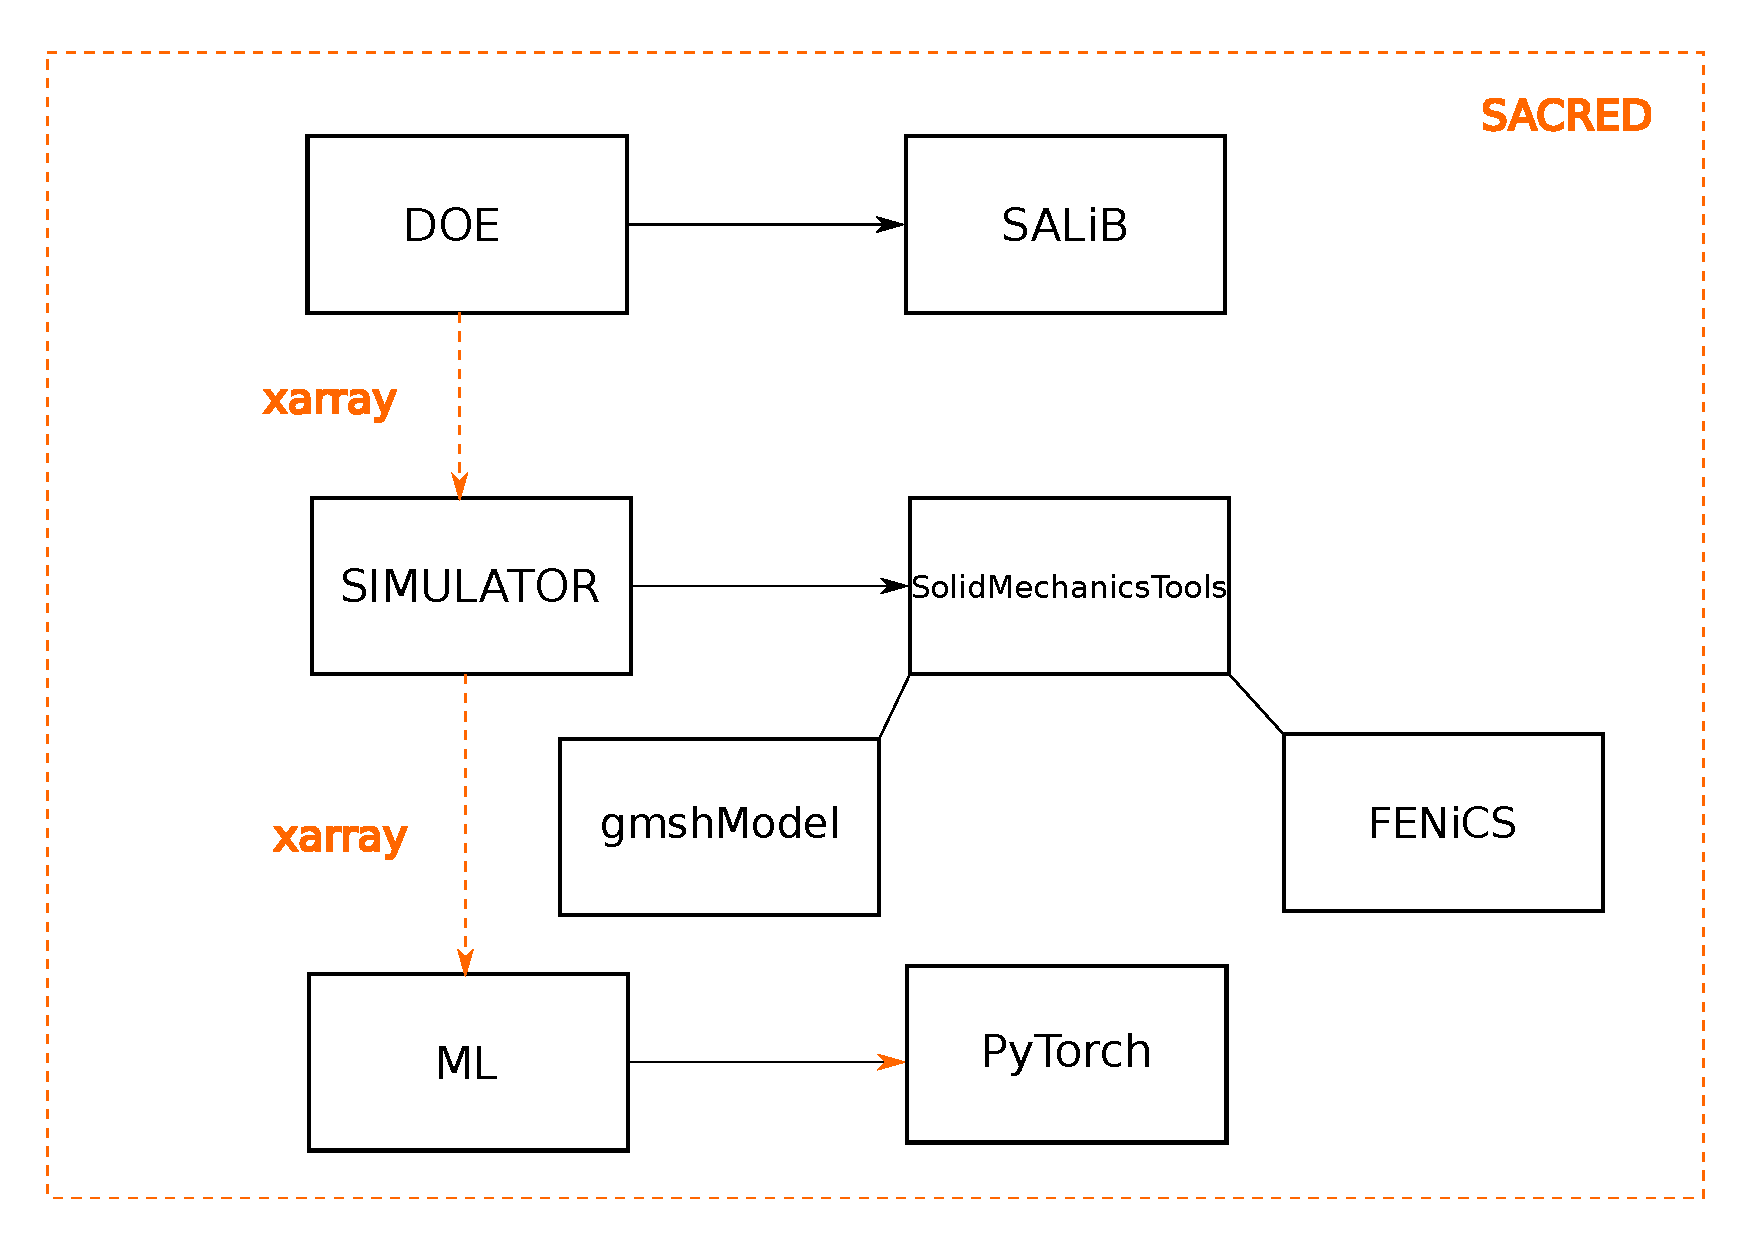
\includegraphics[width=\textwidth]{Figures/DDSCT-flow.pdf}
  \end{minipage}
\end{frame}

\begin{frame}{DDSCT-v0.0.1}
  \begin{minipage}{0.5\textwidth}
    \begin{block}{\color{White} multiprocessing}
  \begin{itemize}
    \item Pool of workers
    \item Not everything is parallelizable.
  \end{itemize}
    \end{block}
  \end{minipage}%
  \begin{minipage}{0.5\textwidth}
    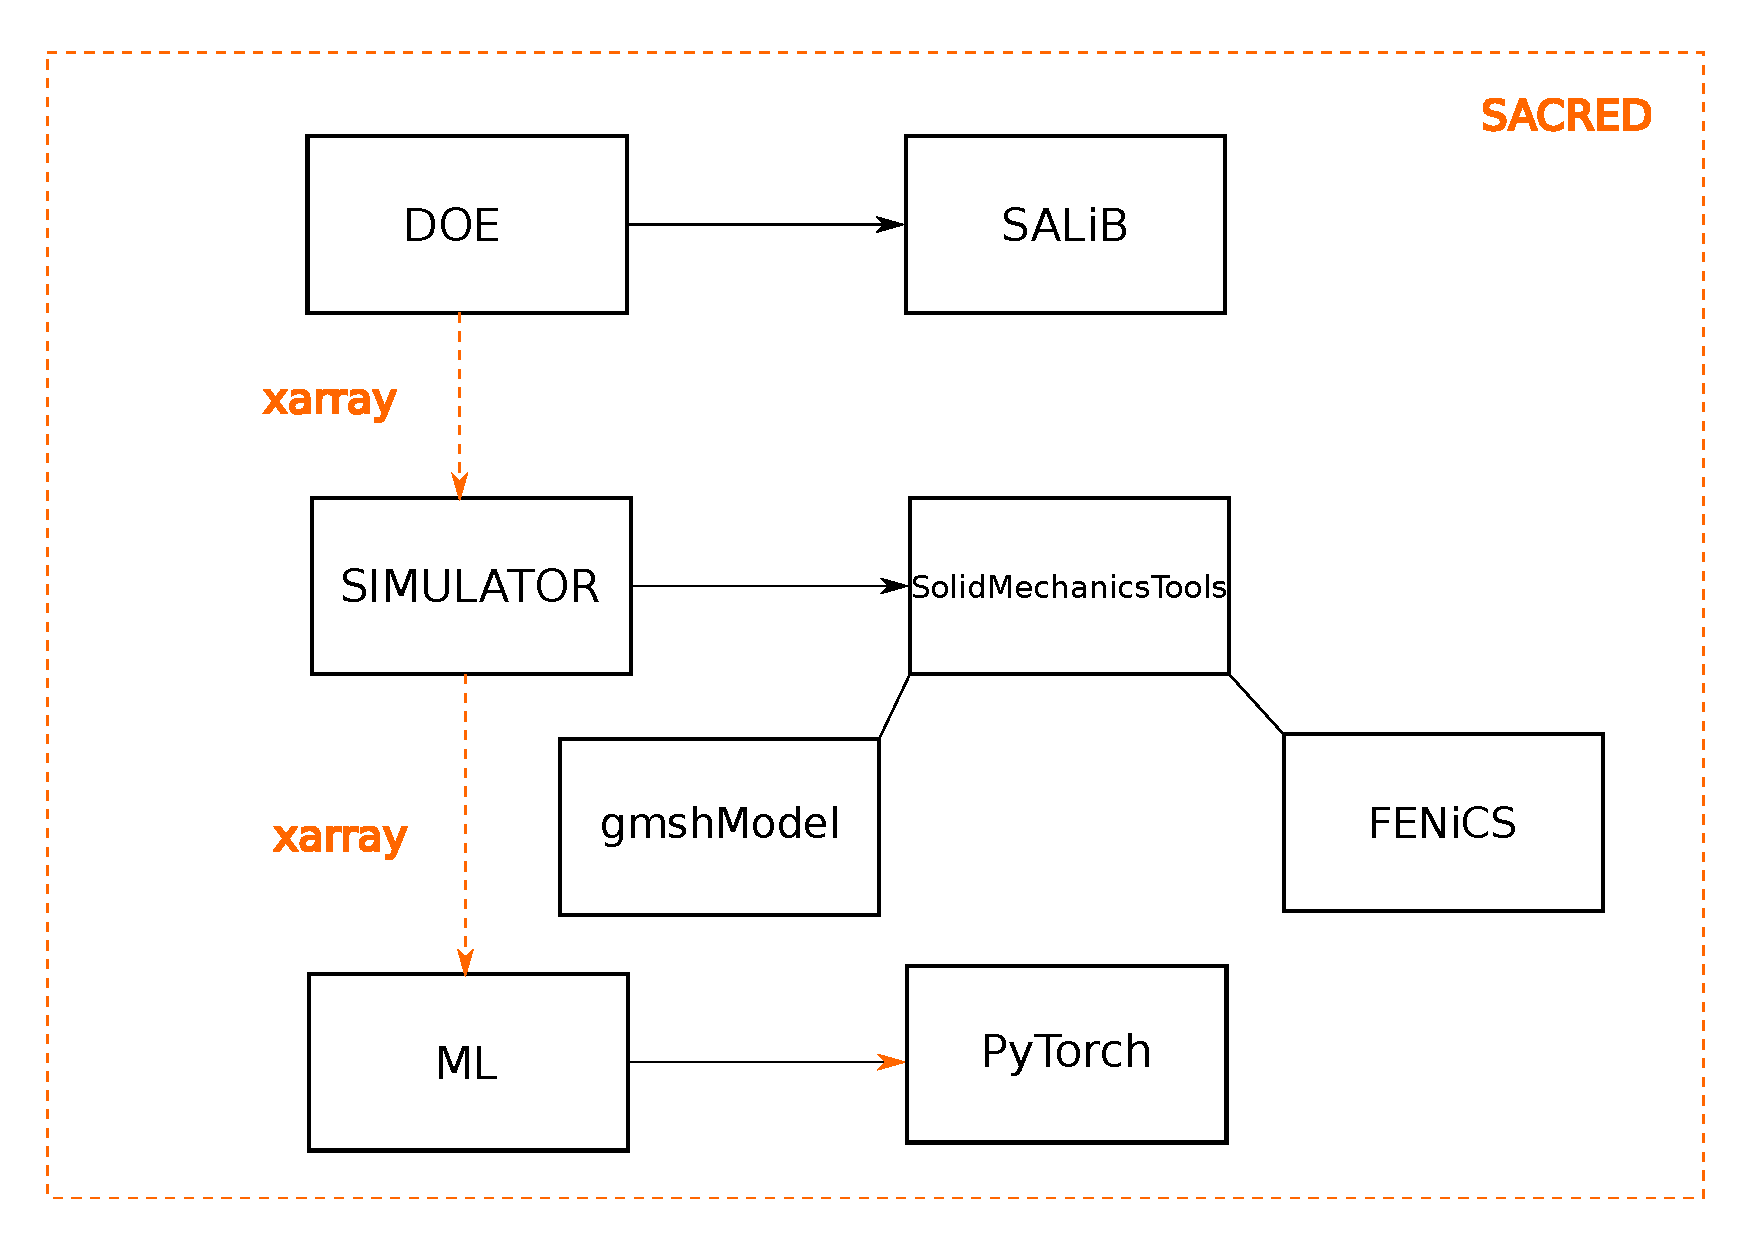
\includegraphics[width=\textwidth]{Figures/DDSCT-flow.pdf}
  \end{minipage}
\end{frame}

\begin{frame}{Final Words}
  \centering
  \begin{itemize}
    \item Shared my ideas/vision with Miguel
    \item Direction towards my ideal, but still specific applications are desired
    \item Please contact Gawel, Shushu or Miguel for information regarding F3DASM
    \item AIM: lightweight starting point for MSc students
  \end{itemize}
\end{frame}

\begin{frame}
  \centering
  \color{Pink}{What are the tools that you think: "Thank god, this exists!!!"?}
\end{frame}

\end{document}

